\chapter{Evaluation}

In this chapter, we will evaluate the Psnodig tool against the goals we set in Section 1. We will look at the general effort to add a new parser, correctness and performance of our interpreter, and whether or not our writers are able to produce satisfactory output. \\

All the Psnodig examples in this chapter will be created entirely through the command line interface, to ensure that the examples are reproducable. To keep a common thread going through this chapter, as well as keeping it fair to all parts of the tool, there are four algorithms that we will use for evaluation: \texttt{Naive search}, \texttt{Bubble sort}, \texttt{Deletion in a Binary search tree} and \texttt{Depth-first search}.

\subsubsection{Naive search}

Naive search is a simple algorithm where we look for a particular element in a list. It is naive because it iterates the list in a simple start-to-end fashion, without applying any heuristics, contrary to the \textbf{Binary search} algorithm mentioned in Section 2.1.1.

\subsubsection{Bubble sort}

Bubble sort is one of the most straightforward sorting algorithms we have available. It is used to sort a list, making sure that for all elements, the element on the left is smaller, and the element on the right is bigger. Bubble sort is seldom applied to solve real problems, but is a popular algorithm for teaching students about sorting algorithms as a concept. \\

If the input list only contains one element or is empty, we return it as it is. Otherwise, we compare the elements on index 0 and 1, and if the first is larger than the second, we swap them. Then we continue to compare the elements on index 1 and 2, and so on. We do this \textbf{n} times, where \textbf{n} equals the length of the list minus one. In each passing, the unsorted largest element in the list is placed in its proper position towards the end of the list.

\subsubsection{Deletion in a Binary search tree}

Binary search trees are a common data structure in computer science. Each node has at most two child nodes, and all nodes are descendents of a single root node. Additionally, for all nodes \textbf{nd}, every node to the left of \textbf{nd} must have a value smaller than or equal to \textbf{nd}, and every node to the right must have a value greater than or equal to \textbf{nd}. \\

Deletion in a binary search tree involves finding a node with a specific value, and removing it whilst preserving the search tree's properties. There are three cases to consider: deletion of a node with no children, deletion of a node with one child, and deletion of a node with two children. \\

If the node has no children, we can simply remove it. If the node has one child, that child takes the place of its parent. If the node has two children, we substitute it with the right subtree's smallest-value node or the left subtree's largest-value node, before removing the original node.

\subsubsection{Depth-first search}

Depth-first search, also referred to as DFS, is an algorithm for traversing a graph data structure. We begin at an arbitrary node of the graph, and ``visit'' neighbouring nodes, following each path as far as possible. \\

It is commonly used to identify all nodes within a connected component. If the graph we are working with is also unweighted, we can use DFS to find its shortest path.

\section{Extensible}

The first goal of Psnodig is extensibility: we should be able to add parsers that are able to convert source code to an internal representation of Psnodig. We have successfully written a parser for an imperative, C-like programming language that we coined \textbf{Gourmet}.

\subsection{Gourmet parser}

What we aim to evaluate here, is whether or not the parser is compatible with Psnodig. The Psnodig grammar is a limitation of how rich a program can look before it is converted by a writer. This means that a parser can at most parse all data types, but at the very least a `Program`, as it is the entry point of all Psnodig programs. \\

A minimal example is an empty program. The Gourmet parser is capable of parsing empty files, producing an AST of a \texttt{Program Nothing [] [] Nothing} value. We cannot produce a maximal example, because \texttt{Program} contains a list of \texttt{FunctionDecl} values, which again contain a list of \texttt{Statement} values. These values can be compound, and in effect go on forever.\footnote{We could interpret a maximal example to be a program limited by our computer’s memory, but theoretically Psnodig programs can be infinitely big.} \\

To evaluate if we have successfully extended Psnodig with a parser, we will implement the four algorithms. We will then run them on a function that parses the programs, and produces either a Psnodig AST or a parse error. \\

\Cref{naiveSearchGourmet} shows an implementation of Naive search in Gourmet, and \Cref{nsAST} shows the Psnodig AST generated from parsing the program. \\

\forsup{gjør eksemplene pene! bytt ut bst greia, dessverre. men finn noe annet bst-relatert?}

\begin{lstlisting}[caption={Naive search implementation in Gourmet.}, captionpos=b, label={naiveSearchGourmet}]
? A list A and an integer x?
! True if x $\$$\in$\$$ A and false if not!

func NaiveSearch(A list, x int) {
    # n := length(A)
    for i := A {
        if i == x {
            return true
        }
    }
    return false
}
\end{lstlisting}

\begin{lstlisting}[caption={The Psnodig AST generated by parsing \Cref{naiveSearchGourmet}.}, captionpos=b, label={nsAST}]
Program
  (Just (ProgramDescription
    "A list A and an integer x"
    "True if x $\$$\in$\$$ A and false if not"))
  []
  [ FunctionDecl
      "NaiveSearch"
      [ Argument "A" "list", Argument "x" "int" ]
      [ HashStmt
          (Assignment
              (VariableTarget "n")
              (ExpressionValue
                (CallExp
                    (FunctionCall "length" [VariableExp "A"])))
          ),
        ForEach
          "i"
          (VariableExp "A")
          [ If
              (BinaryExp Equal
                (VariableExp "i")
                (VariableExp "x"))
              [Return (Constant (Boolean True))]
              Nothing
          ],
        Return (Constant (Boolean False))
      ]
  ]
  Nothing
\end{lstlisting}

\Cref{bubbleSortGourmet} shows an implementation of Bubble sort in Gourmet, and \Cref{bsAST} shows the Psnodig AST generated from parsing the program. \\

\begin{lstlisting}[caption={Bubble sort implementation in Gourmet.}, captionpos=b, label={bubbleSortGourmet}]
? A list A?
! The list A, but ordered from smallest value to largest!

func BubbleSort(A list) {
    # n := length(A)
    for i := 0, n - 2 {
        for j := 0, n - i - 2 {
            if A[j] > A[j+1] {
                @{swap A[j] with A[j+1]}{
                    tmp := A[j]
                    A[j] := A[j+1]
                    A[j+1] := tmp
                }
            }
        }
    }
    return A
}
\end{lstlisting}

\begin{lstlisting}[caption={The Psnodig AST generated by parsing \Cref{bubbleSortGourmet}.}, captionpos=b, label={bsAST}]
Program
  ( Just
      ( ProgramDescription
          "A list A"
          "The list A, but ordered from smallest value to largest"
      )
  )
  []
  [ FunctionDecl
      "BubbleSort"
      [Argument "A" "list"]
      [ HashStmt
          ( Assignment
              (VariableTarget "n")
              ( ExpressionValue
                  ( CallExp
                      (FunctionCall "length" [VariableExp "A"])
                  )
              )
          ),
        For
          "i"
          (Constant (Number 0))
          ( BinaryExp
              Minus
              (VariableExp "n")
              (Constant (Number 1))
          )
          [ For
              "j"
              (Constant (Number 0))
              ( BinaryExp
                  Minus
                  ( BinaryExp
                      Minus
                      (VariableExp "n")
                      (VariableExp "i")
                  )
                  (Constant (Number 1))
              )
              [ If
                  ( BinaryExp
                      GreaterThan
                      (ListIndex "A" [VariableExp "j"])
                      ( ListIndex
                          "A"
                          [ BinaryExp
                              Plus
                              (VariableExp "j")
                              (Constant (Number 1))
                          ]
                      )
                  )
                  [ AnnotationStmt
                      "swap A[j] with A[j+1]"
                      [ Assignment
                          (VariableTarget "tmp")
                          ( ExpressionValue
                              (ListIndex "A" [VariableExp "j"])
                          ),
                        Assignment
                          (ListIndexTarget "A" [VariableExp "j"])
                          ( ExpressionValue
                              ( ListIndex
                                  "A"
                                  [ BinaryExp
                                      Plus
                                      (VariableExp "j")
                                      (Constant (Number 1))
                                  ]
                              )
                          ),
                        Assignment
                          ( ListIndexTarget
                              "A"
                              [ BinaryExp
                                  Plus
                                  (VariableExp "j")
                                  (Constant (Number 1))
                              ]
                          )
                          (ExpressionValue (VariableExp "tmp"))
                      ]
                  ]
                  Nothing
              ]
          ],
        Return (VariableExp "A")
      ]
  ]
  Nothing
\end{lstlisting}

\Cref{deleteBSTGourmet} shows an implementation of Deletion in a binary tree in Gourmet, and \Cref{dbstAST} shows the Psnodig AST generated from parsing the program. \\

\begin{lstlisting}[caption={Deletion in a binary search tree implementation in Gourmet.}, captionpos=b, label={deleteBSTGourmet}]
? The root node in a tree and the value of a node to be deleted?
! The updated tree with one less node!

struct Tree {
    value int,
    left Tree,
    right Tree
}

func Delete(node Tree, val int) {
    if node == nil {
        return nil
    }
    else if (node.value) < val {
        node.right := Delete(node.right, val)
        return node
    }
    else if (node.value) > val {
        node.left := Delete(node.left, val)
        return node
    }

    if (node.left) == nil {
        return node.right
    }
    else if (node.right) == nil {
        return node.left
    }

    node' := FindMax(node.left)
    node.value := node'.value
    node.left := Delete(node.left, node.value)
    return node
}

func FindMax(root Tree) {
    if (root.right) == nil {
        return (root.value)
    }

    return FindMax(root.right)
}
\end{lstlisting}

\begin{lstlisting}[caption={The Psnodig AST generated by parsing \Cref{deleteBSTGourmet}.}, captionpos=b, label={dbstAST}]
Program (Just (ProgramDescription "The root node in a tree and the value of a node to be deleted" "The updated tree with one less node")) [StructDecl "Tree" [Argument "value" "int",Argument "left" "Tree",Argument "right" "Tree"]] [FunctionDecl "Delete" [Argument "node" "Tree",Argument "val" "int"] [If (BinaryExp Equal (VariableExp "node") (Constant Nil)) [Return (Constant Nil)] (Just (ElseIf (BinaryExp LessThan (StructFieldExp (StructField (VariableExp "node") (VariableExp "value"))) (VariableExp "val")) [Assignment (StructFieldTarget (StructField (VariableExp "node") (VariableExp "right"))) (ExpressionValue (CallExp (FunctionCall "Delete" [StructFieldExp (StructField (VariableExp "node") (VariableExp "right")),VariableExp "val"]))),Return (VariableExp "node")] (Just (ElseIf (BinaryExp GreaterThan (StructFieldExp (StructField (VariableExp "node") (VariableExp "value"))) (VariableExp "val")) [Assignment (StructFieldTarget (StructField (VariableExp "node") (VariableExp "left"))) (ExpressionValue (CallExp (FunctionCall "Delete" [StructFieldExp (StructField (VariableExp "node") (VariableExp "left")),VariableExp "val"]))),Return (VariableExp "node")] Nothing)))),If (BinaryExp Equal (StructFieldExp (StructField (VariableExp "node") (VariableExp "left"))) (Constant Nil)) [Return (StructFieldExp (StructField (VariableExp "node") (VariableExp "right")))] (Just (ElseIf (BinaryExp Equal (StructFieldExp (StructField (VariableExp "node") (VariableExp "right"))) (Constant Nil)) [Return (StructFieldExp (StructField (VariableExp "node") (VariableExp "left")))] Nothing)),Assignment (VariableTarget "node'") (ExpressionValue (CallExp (FunctionCall "FindMax" [StructFieldExp (StructField (VariableExp "node") (VariableExp "left"))]))),Assignment (StructFieldTarget (StructField (VariableExp "node") (VariableExp "value"))) (ExpressionValue (StructFieldExp (StructField (VariableExp "node'") (VariableExp "value")))),Assignment (StructFieldTarget (StructField (VariableExp "node") (VariableExp "left"))) (ExpressionValue (CallExp (FunctionCall "Delete" [StructFieldExp (StructField (VariableExp "node") (VariableExp "left")),StructFieldExp (StructField (VariableExp "node") (VariableExp "value"))]))),Return (VariableExp "node")],FunctionDecl "FindMax" [Argument "root" "Tree"] [If (BinaryExp Equal (StructFieldExp (StructField (VariableExp "root") (VariableExp "right"))) (Constant Nil)) [Return (StructFieldExp (StructField (VariableExp "root") (VariableExp "value")))] Nothing,Return (CallExp (FunctionCall "FindMax" [StructFieldExp (StructField (VariableExp "root") (VariableExp "right"))]))]] Nothing
\end{lstlisting}

\Cref{dfsGourmet} shows an implementation of Naive search in Gourmet, and \Cref{dfsAST} shows the Psnodig AST generated from parsing the program. \\

\begin{lstlisting}[caption={DFS implementation in Gourmet.}, captionpos=b, label={dfsGourmet}]
? A list of booleans, a stack of nodes, a graph and a starting node?
! The list of booleans!

func dfs(visited list, stack list, graph list, node int) {
    add(node, visited)
    append(node, stack)

    while length(stack) > 0 {
        m := pop(stack)

        for nb := get(m, graph) {
            if not in(nb, visited) {
                add(nb, visited)
                append(nb, stack)
            }
        }
    }
    return visited
}
\end{lstlisting}

\begin{lstlisting}[caption={The Psnodig AST generated by parsing \Cref{dfsGourmet}.}, captionpos=b, label={dfsAST}]
Program
    (Just (ProgramDescription "A list of booleans, a stack of nodes, a graph and a starting node" "The list of booleans"))
    []
    [FunctionDecl "dfs" [Argument "visited" "list", Argument "stack" "list", Argument "graph" "list", Argument "node" "int"] [CallStmt (FunctionCall "add" [VariableExp "node", VariableExp "visited"]), CallStmt (FunctionCall "append" [VariableExp "node", VariableExp "stack"]), Loop (BinaryExp GreaterThan (CallExp (FunctionCall "length" [VariableExp "stack"])) (Constant (Number 0))) [Assignment (VariableTarget "m") (ExpressionValue (CallExp (FunctionCall "pop" [VariableExp "stack"]))), ForEach "nb" (CallExp (FunctionCall "get" [VariableExp "m", VariableExp "graph"])) [If (Not (CallExp (FunctionCall "in" [VariableExp "nb", VariableExp "visited"]))) [CallStmt (FunctionCall "add" [VariableExp "nb", VariableExp "visited"]), CallStmt (FunctionCall "append" [VariableExp "nb", VariableExp "stack"])] Nothing]], Return (VariableExp "visited")]]
    Nothing
\end{lstlisting}

\section{Executable}

The second goal from Section 1 was that our tool should be executable. Therefore, Psnodig comes with an interpreter working directly on the internal representation. When a parser has successfully converted a source program to Psnodig, we want to be able to run that code. This way, no matter what langauge we use to write our program, it is the converted version that is ultimately executed. \\

Naturally, we would like all programs to be executable. However, the interpreter currently stands without an implementation for the statement types \textbf{Break} and \textbf{Continue}. If a program flow runs into either of them, the program will terminate with a warning. Except for these, all Psnodig data types are handled by the interpreter. \\

Now we can try to execute the programs we mentioned earlier. We use the Gourmet programs from earlier to give us the internal representation, rather than constructing them ourselves through variables, because we believed them to be satisfactory.

\section{Presentable}

\forsup{se på goals igjen. gourmet og python er faktisk deler av exteisble, ikke executable. presentable handler utelukkende om tbp og ibp. python writer brukes kinda som benchmark for å se hvor mye effort det er å lage python parser (kan sammenligne gourmet parser og writer her)}

\subsection{Gourmet writer}

The last part of our evaluation is the set of writers we currently have available. We will evaluate all four individually, and we start with the Gourmet writer. This is the one where flaws are easiest to locate, as the output programs should be more or less 1-to-1 with the source programs. \\

\Cref{naiveSearchGourmet2}, \Cref{bubbleSortGourmet2}, \Cref{deleteBSTGourmet2}, and \Cref{dfsGourmet2} show the results of transpiling Gourmet back to Gourmet. The only real difference is the amount of whitespace in some areas, and by executing the transpiled results we get the same results as before. \\

\begin{lstlisting}[caption={The result of transpiling \Cref{naiveSearchGourmet} back to Gourmet.}, captionpos=b, label={naiveSearchGourmet2}]
? A list $A$ and an integer $x$ ?
! True if $x \in A$ and false if not !

func NaiveSearch(A list, x int) {
	# n := length(A)
	for i := A {
		if i == x {
			return true
		}
	}
	return false
}
\end{lstlisting}

\begin{lstlisting}[caption={The result of transpiling \Cref{bubbleSortGourmet} back to Gourmet.}, captionpos=b, label={bubbleSortGourmet2}]
? A list $A$ ?
! The list $A$, but ordered from smallest value to largest !

func BubbleSort(A list) {
	# n := length(A)
	for i := 0, n - 1 {
		for j := 0, n - i - 1 {
			if A[j] > A[j + 1] {
				@{swap A[j] with A[j+1]}{
					tmp := A[j]
					A[j] := A[j + 1]
					A[j + 1] := tmp
				}
			}
		}
	}
	return A
}
\end{lstlisting}

\begin{lstlisting}[caption={The result of transpiling \Cref{deleteBSTGourmet} back to Gourmet.}, captionpos=b, label={deleteBSTGourmet2}]
? The root node in a tree and the value of a node to be deleted ?
! The updated tree with one less node !

struct Tree {
	value int,
	left Tree,
	right Tree
}

func Delete(node Tree, val int) {
	if node == nil {
		return nil
	} else if node.value < val {
		node.right := Delete(node.right, val)
		return node
	} else if node.value > val {
		node.left := Delete(node.left, val)
		return node
	}
	if node.left == nil {
		return node.right
	} else if node.right == nil {
		return node.left
	}
	node' := FindMax(node.left)
	node.value := node'.value
	node.left := Delete(node.left, node.value)
	return node
}

func FindMax(root Tree) {
	if root.right == nil {
		return root.value
	}
	return FindMax(root.right)
}
\end{lstlisting}

\begin{lstlisting}[caption={The result of transpiling \Cref{dfsGourmet} back to Gourmet.}, captionpos=b, label={dfsGourmet2}]
? A list of booleans, a stack of nodes, a graph and a starting node?
! The list of booleans!

func dfs(visited list, stack list, graph list, node int) {
    visited[node] := true
    append(node, stack)

    while length(stack) > 0 {
        m := pop(stack)
        print(m)

        for nb := get(m, graph) {
            if visited[nb] == false {
                visited[nb] := true
                append(nb, stack)
            }
        }
    }
    return visited
}
\end{lstlisting}

\subsection{Python writer}

The next writer we evaluate is the Python writer. The output will be relatively similar to Gourmet, since the latter also employs indentation. However,  \\

\Cref{naiveSearchPython}, \Cref{bubbleSortPython}, \Cref{deleteBSTPython}, and \Cref{dfsPython} show the results of transpiling Gourmet to Python. There are syntactic differences, like using colons over curly braces, and writing hash- and annotation statements like regular statements. We also see structs being replaced by classes, and Psnodig functions being replaced by Python ones. \\

\begin{lstlisting}[caption={The result of transpiling \Cref{naiveSearchGourmet} to Python.}, captionpos=b, label={naiveSearchPython}]
# Input: A list $A$ and an integer $x$
# Output: True if $x \in A$ and false if not

def NaiveSearch(A, x: int):
    n = len(A)
    for i in A:
        if i == x:
            return True


    return False
\end{lstlisting}

\begin{lstlisting}[caption={The result of transpiling \Cref{bubbleSortGourmet} to Python.}, captionpos=b, label={bubbleSortPython}]
# Input: A list $A$
# Output: The list $A$, but ordered from smallest value to largest

def BubbleSort(A):
    n = len(A)
    for i in range(0, n - 1):
        for j in range(0, n - i - 1):
            if A[j] > A[j + 1]:
                tmp = A[j]
                A[j] = A[j + 1]
                A[j + 1] = tmp




    return A
\end{lstlisting}

\begin{lstlisting}[caption={The result of transpiling \Cref{deleteBSTGourmet} to Python.}, captionpos=b, label={deleteBSTPython}]
# Input: The root node in a tree and the value of a node to be deleted
# Output: The updated tree with one less node

class Tree:
    def __init__(self, value, left, right):
        self.value = value
        self.left = left
        self.right = right


def Delete(node, val: int):
    if node == None:
        return None
    elif node.value < val:
        node.right = Delete(node.right, val)
        return node
    elif node.value > val:
        node.left = Delete(node.left, val)
        return node

    if node.left == None:
        return node.right
    elif node.right == None:
        return node.left

    node' = FindMax(node.left)
    node.value = node'.value
    node.left = Delete(node.left, node.value)
    return node


def FindMax(root):
    if root.right == None:
        return root.value

    return FindMax(root.right)
\end{lstlisting}

\begin{lstlisting}[caption={The result of transpiling \Cref{dfsGourmet} to Python.}, captionpos=b, label={dfsPython}]
# Input: A list of booleans, a stack of nodes, a graph and a starting node
# Output: The list of booleans

def dfs(visited, stack, graph, node: int):
    visited[node] = True
    stack.append(node)
    while len(stack) > 0:
        m = stack.pop()
        print(m)
        for nb in graph[m]:
            if visited[nb] == False:
                visited[nb] = True
                stack.append(nb)



    return visited
\end{lstlisting}

As an extra test to see if we really are able to transpile programs to syntactically correct Python equivalents, we will run the final transpiled code with the Python interpreter, and compare the results with those of the Psnodig interpreter. \\

\forsup{men hvordan presentere det??}

\subsection{Pseudocode writer}

The pseudocode writer converts the intermediate representation to a much different abstraction level than we saw in the two previous writers. Now, the code is no longer executable. \\

This writer gives us a LaTeX file, accompanied by the compiled result in a PDF if we wish. In this section, however, we will ignore the LaTeX file, and solely view the compiled versions. \\

\Cref{naiveSearchTBP}, \Cref{bubbleSortTBP}, \Cref{deleteBSTTBP}, and \Cref{dfsTBP} show the results of transpiling Gourmet to TBP. \\

\begin{figure}[ht!]
    \centering
    \includegraphics[scale=.95]{assets/chapter6/NaiveSearchTBP.pdf}
    \caption{The result of transpiling \Cref{naiveSearchGourmet} to pseudocode.}
    \label{naiveSearchTBP}
\end{figure}

\begin{figure}[ht!]
    \centering
    \includegraphics[scale=.95]{assets/chapter6/BubbleSortTBP.pdf}
    \caption{The result of transpiling \Cref{bubbleSortGourmet} to pseudocode.}
    \label{bubbleSortTBP}
\end{figure}

\begin{figure}[ht!]
    \centering
    \includegraphics[scale=.95]{assets/chapter6/DeleteTBP.pdf}
    \caption{The result of transpiling \Cref{deleteBSTGourmet} to pseudocode.}
    \label{deleteBSTTBP}
\end{figure}

\begin{figure}[ht!]
    \centering
    \includegraphics[scale=.95]{assets/chapter6/DFSTBP.pdf}
    \caption{The result of transpiling \Cref{dfsGourmet} to pseudocode.}
    \label{dfsTBP}
\end{figure}

\subsection{Flowchart writer}

The flowchart writer is the most advanced of the four, working on yet another level of abstraction. While the pseudocode writer produces TBP, which at least resembles executable code, the IBP we produce here does not. Whilst expressions are fitted into boxes, control flow statemenets like loops and ifs risk colliding when nested. \\

\Cref{naiveSearchIBP}, \Cref{bubbleSortIBP}, \Cref{deleteBSTIBP}, and \Cref{dfsIBP} show the results of transpiling Gourmet to flowcharts. \\

\begin{figure}[ht!]
    \centering
    \includegraphics[scale=.75]{assets/chapter6/NaiveSearchIBP.pdf}
    \caption{The result of transpiling \Cref{naiveSearchGourmet} to a flowchart.}
    \label{naiveSearchIBP}
\end{figure}

\begin{figure}[ht!]
    \centering
    \includegraphics[scale=.75]{assets/chapter6/BubbleSortIBP.pdf}
    \caption{The result of transpiling \Cref{bubbleSortGourmet} to a flowchart.}
    \label{bubbleSortIBP}
\end{figure}

\begin{figure}[ht!]
    \centering
    \includegraphics[scale=.5]{assets/chapter6/DeleteIBP.pdf}
    \caption{The result of transpiling \Cref{deleteBSTGourmet} to a flowchart.}
    \label{deleteBSTIBP}
\end{figure}

\begin{figure}[ht!]
    \centering
    \includegraphics[scale=.75]{assets/chapter6/DFSIBP.pdf}
    \caption{The result of transpiling \Cref{dfsGourmet} to a flowchart.}
    \label{dfsIBP}
\end{figure}

%\forsup{when we have a lot of text in expression, the boxes grow horizontally, becoming wider and potentially crashing in others. why can’t it grow vertically, and instead just become longer? that way, it won’t really crash in anything!}

%Listing ? And ? show blabla reproduced to the best of our abilities with Code2Flow. Here we see how this and that could be dealt with. \\

%\forsup{`dealt with` er kanskje for uformelt?}

%\forsup{pauze}

%One of few editors that generates flowcharts directly from code is Code2Flow\footnote{Can be found at \url{https://app.code2flow.com/}}. This is a DSL with support for most common programming concepts like statements, loops, conditionals, and more. Functions are put within frames. The editor comes with a comprehensible guide on its syntax. It is also a highly customisable tool: it lets us change the flowcharts' fonts, colours, sizes and even edge height. The free version lets us use at most 50 nodes per flowchart, and we can save up to 5 flowcharts in our account. \\

%\Cref{FizzBuzz written with Code2Flow.} shows a solution to the \texttt{FizzBuzz} problem, commonly presented in entry level interview settings and beginner programming exercises. \Cref{The corresponding flowchart chapter2.} shows the corresponding flowchart we are given by Code2Flow. \\

%\begin{lstlisting}[caption={FizzBuzz written with Code2Flow.}, captionpos=b, label={FizzBuzz written with Code2Flow.}]
%function FizzBuzz (n int) {
 % if (n % 15 == 0) {
  %  print("FizzBuzz")
  %}
  %else if (n % 3 == 0) {
  %  print("Fizz")
  %}
  %else if (n % 5 == 0) {
  %  print("Buzz")
  %}
  %else {
   % print(n)
  %}
%}
%\end{lstlisting}

%\begin{figure}[ht!]
 %   \centering
  %  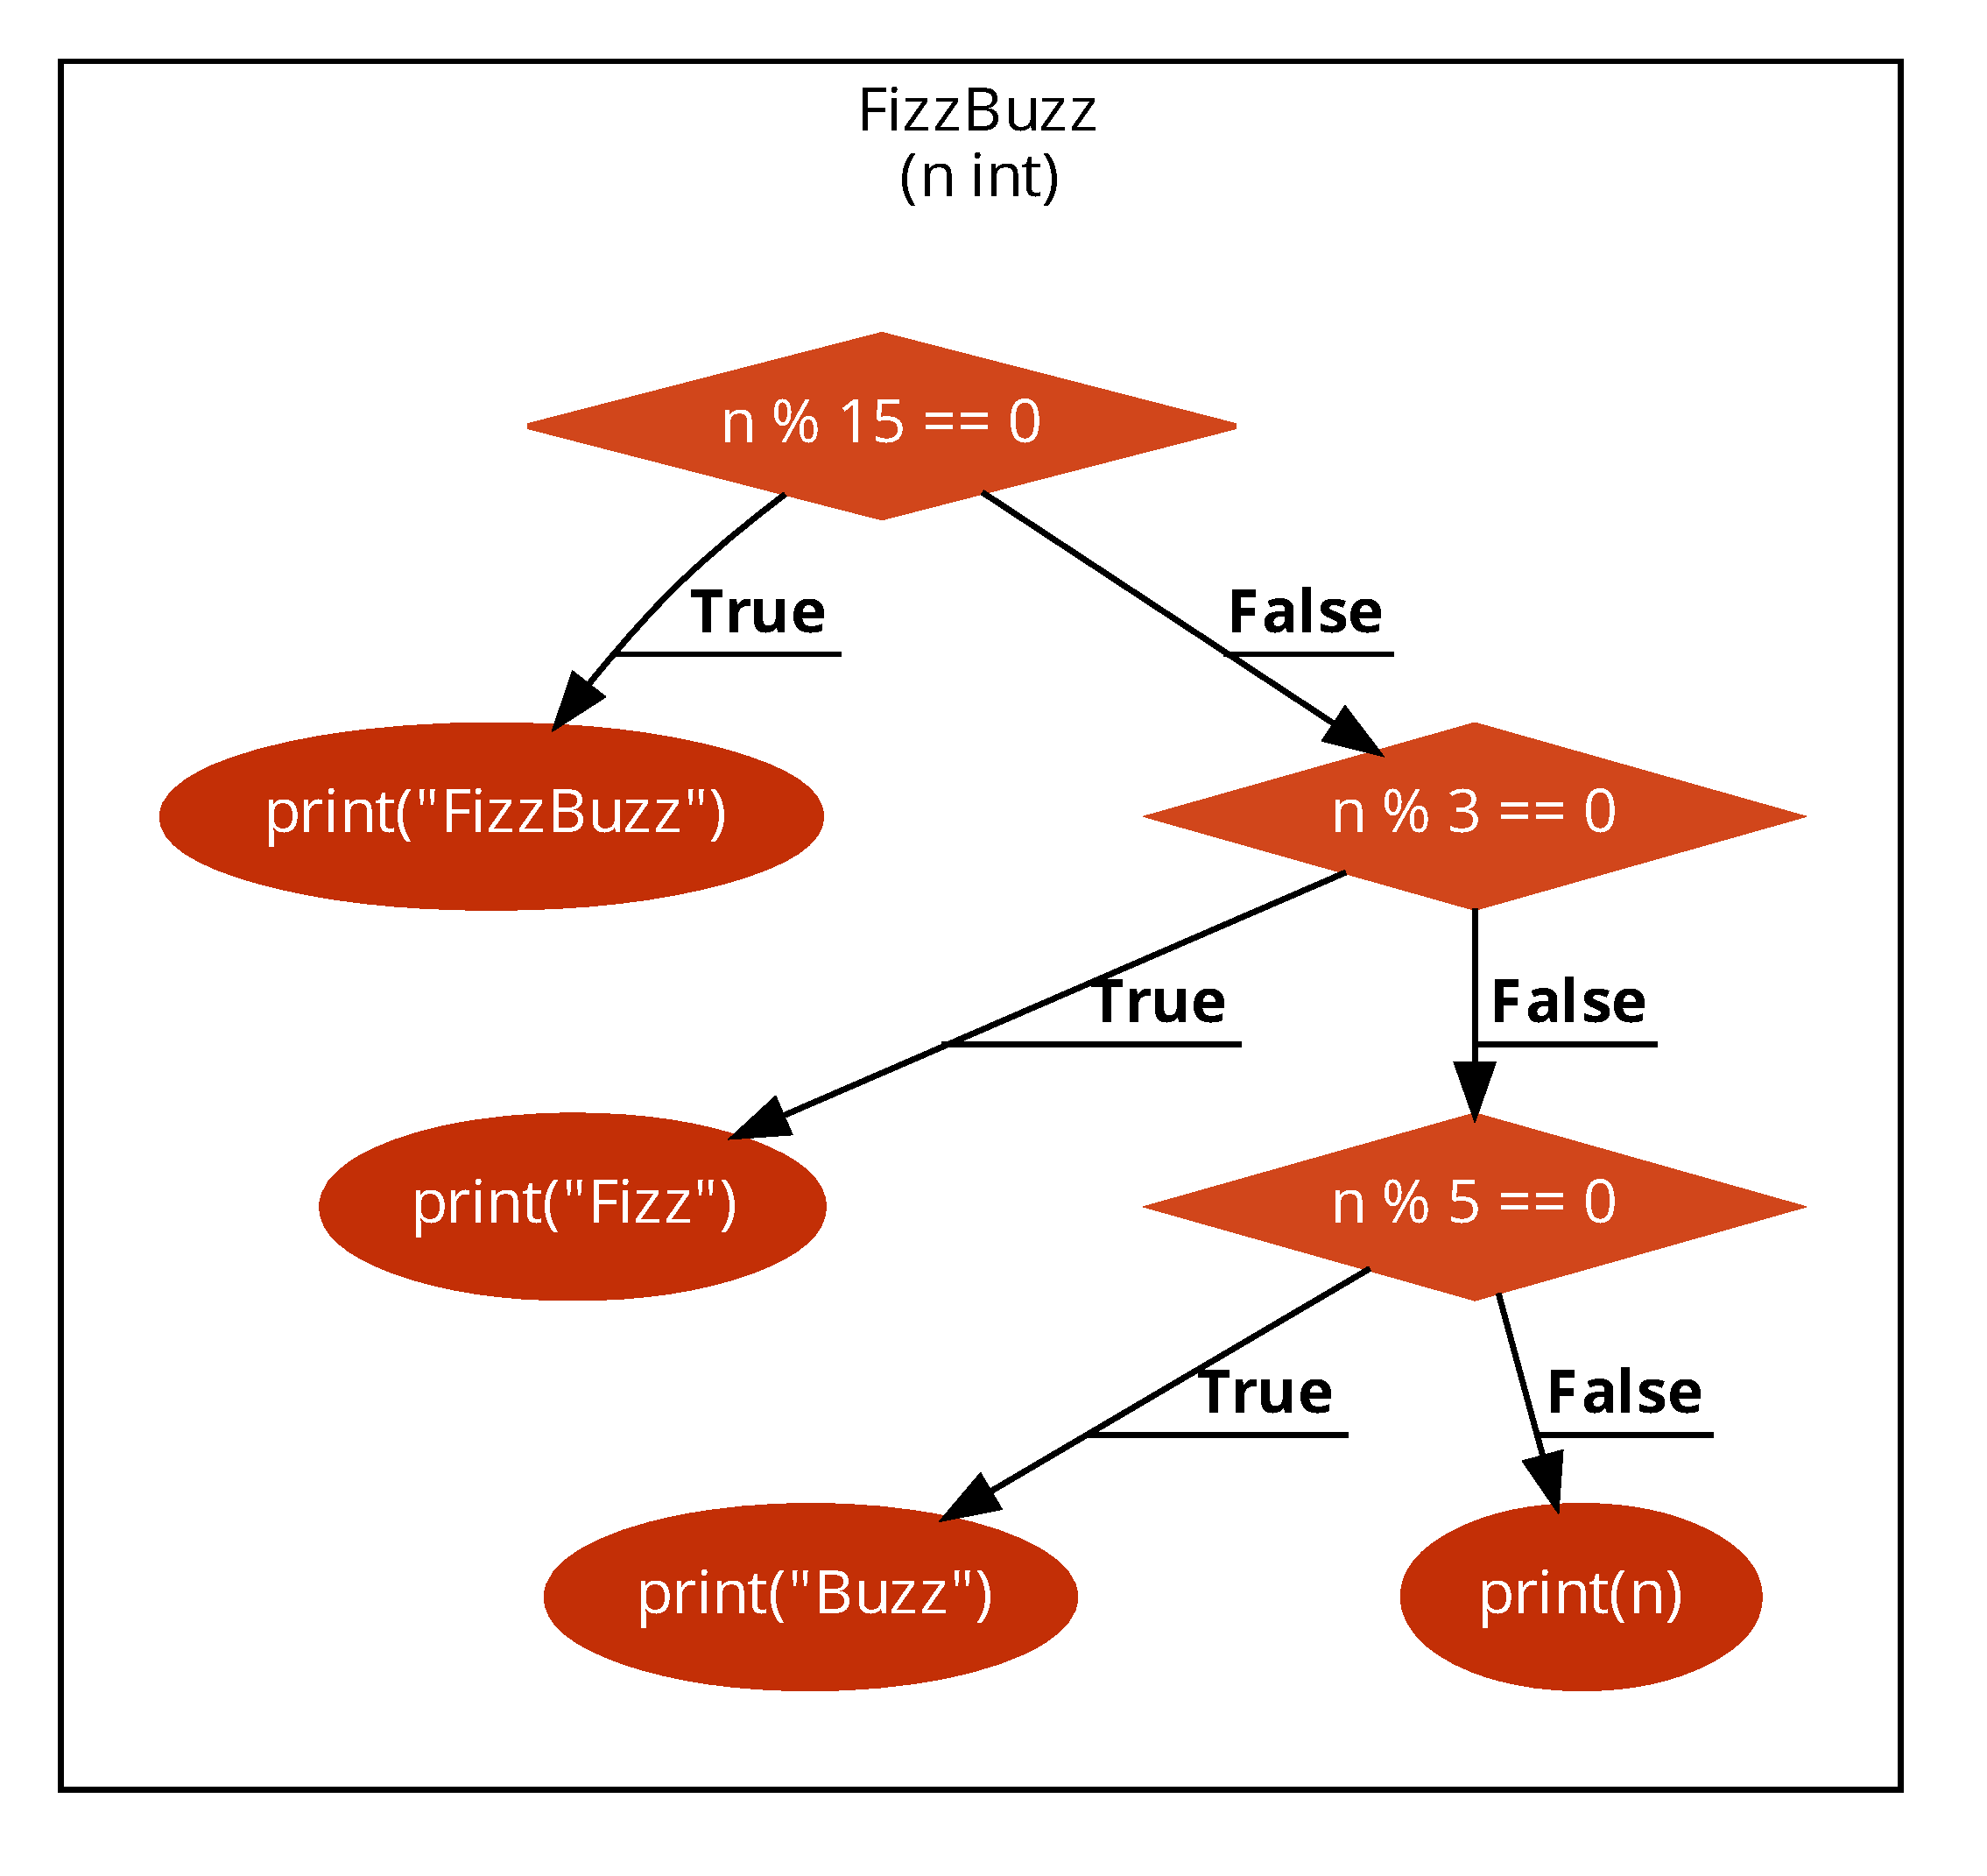
\includegraphics[scale=.2]{assets/chapter2/FizzBuzzCode2Flow.pdf}
   % \caption{The corresponding flowchart to \Cref{FizzBuzz written with Code2Flow.}.}
   % \label{The corresponding flowchart chapter2.}
%\end{figure}
